\begin{apendicesenv}

\partapendices

\chapter{Imagens do Robô}
\label{imagens}

\begin{figure}[h]
    \centering
    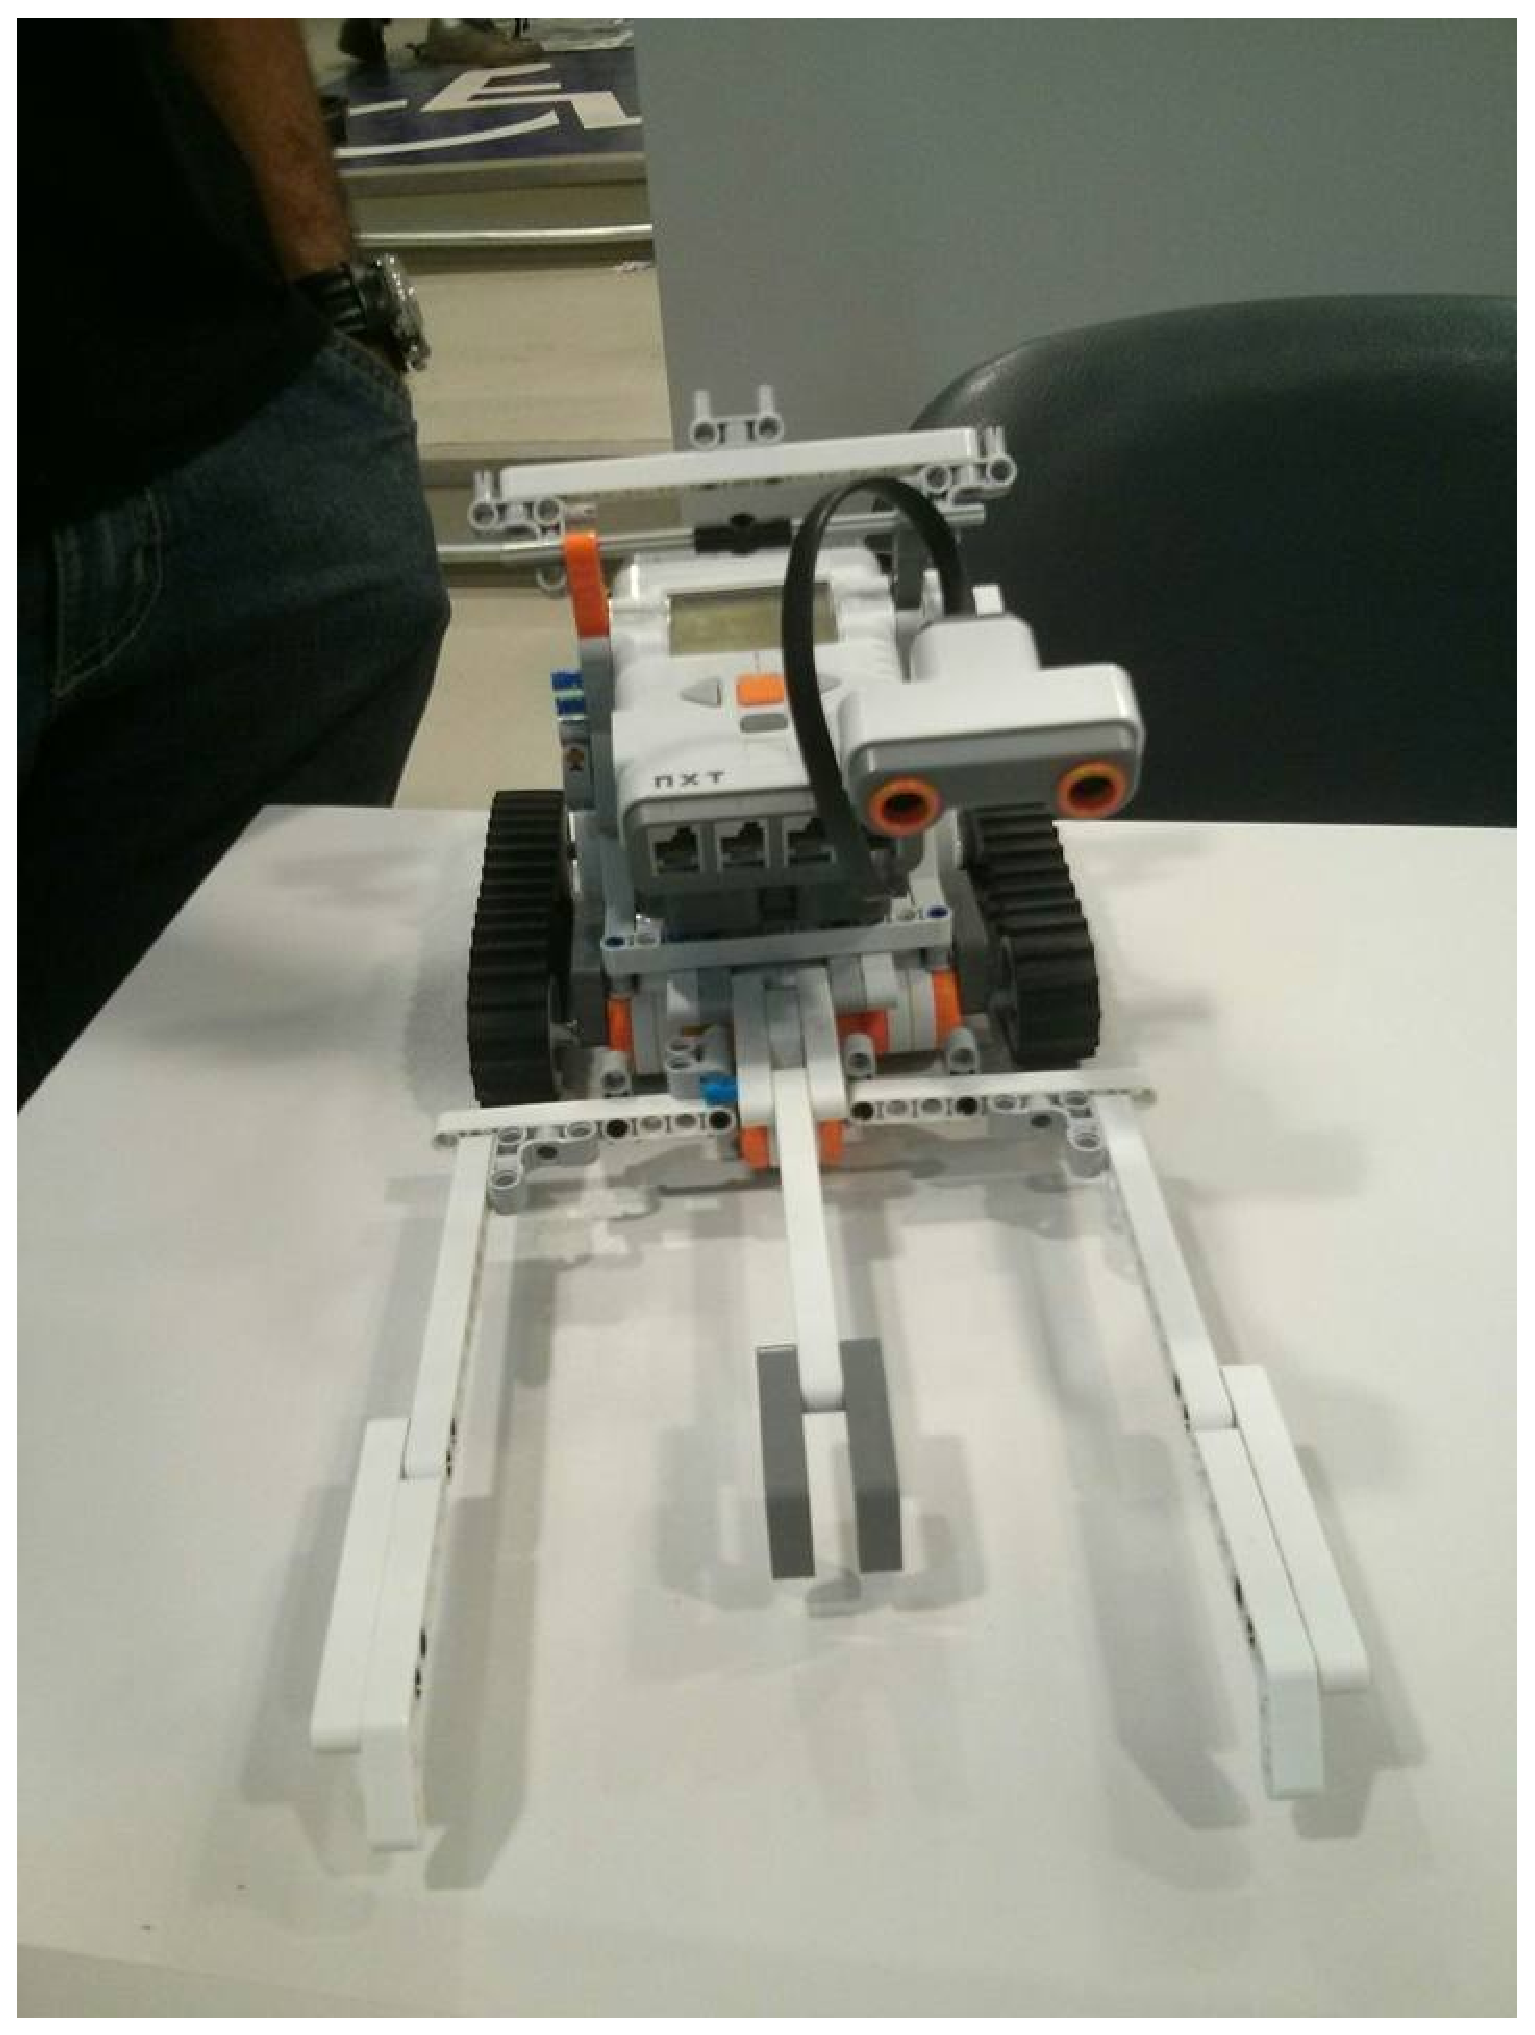
\includegraphics[keepaspectratio=true,scale=0.55]
      {figuras/robo_001.eps}
    \caption{Vista frontal superior.}
\end{figure}

\begin{figure}[h]
    \centering
    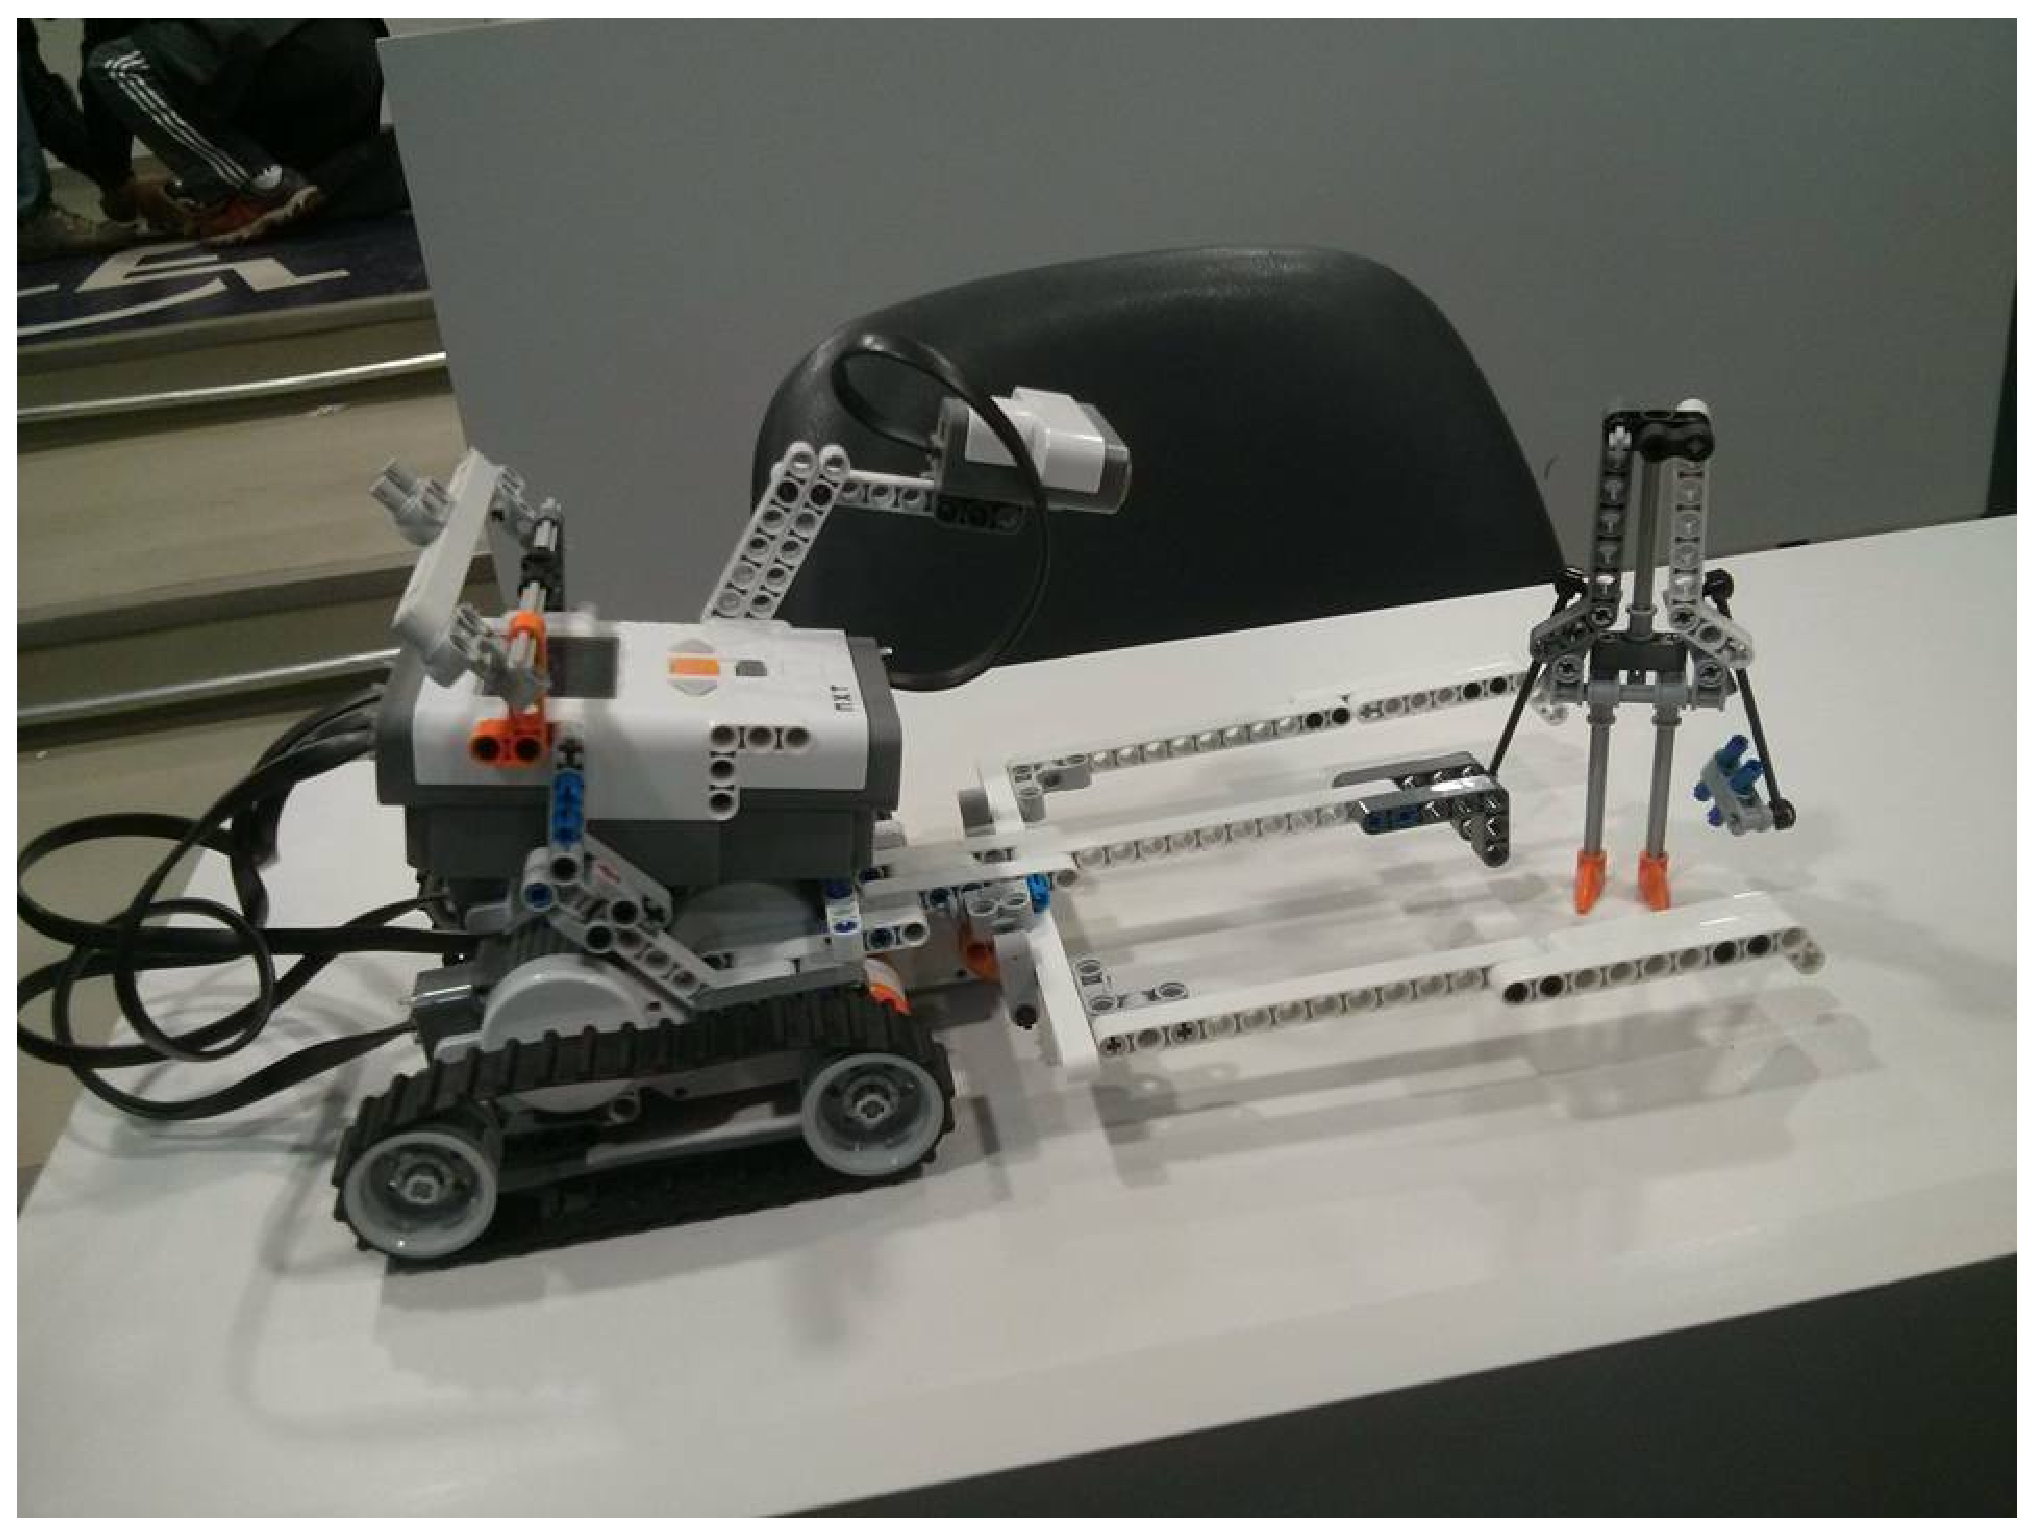
\includegraphics[keepaspectratio=true,scale=0.55]
      {figuras/robo_003.eps}
    \caption{Vista lateral esquerda.}
\end{figure}

\begin{figure}[h]
    \centering
    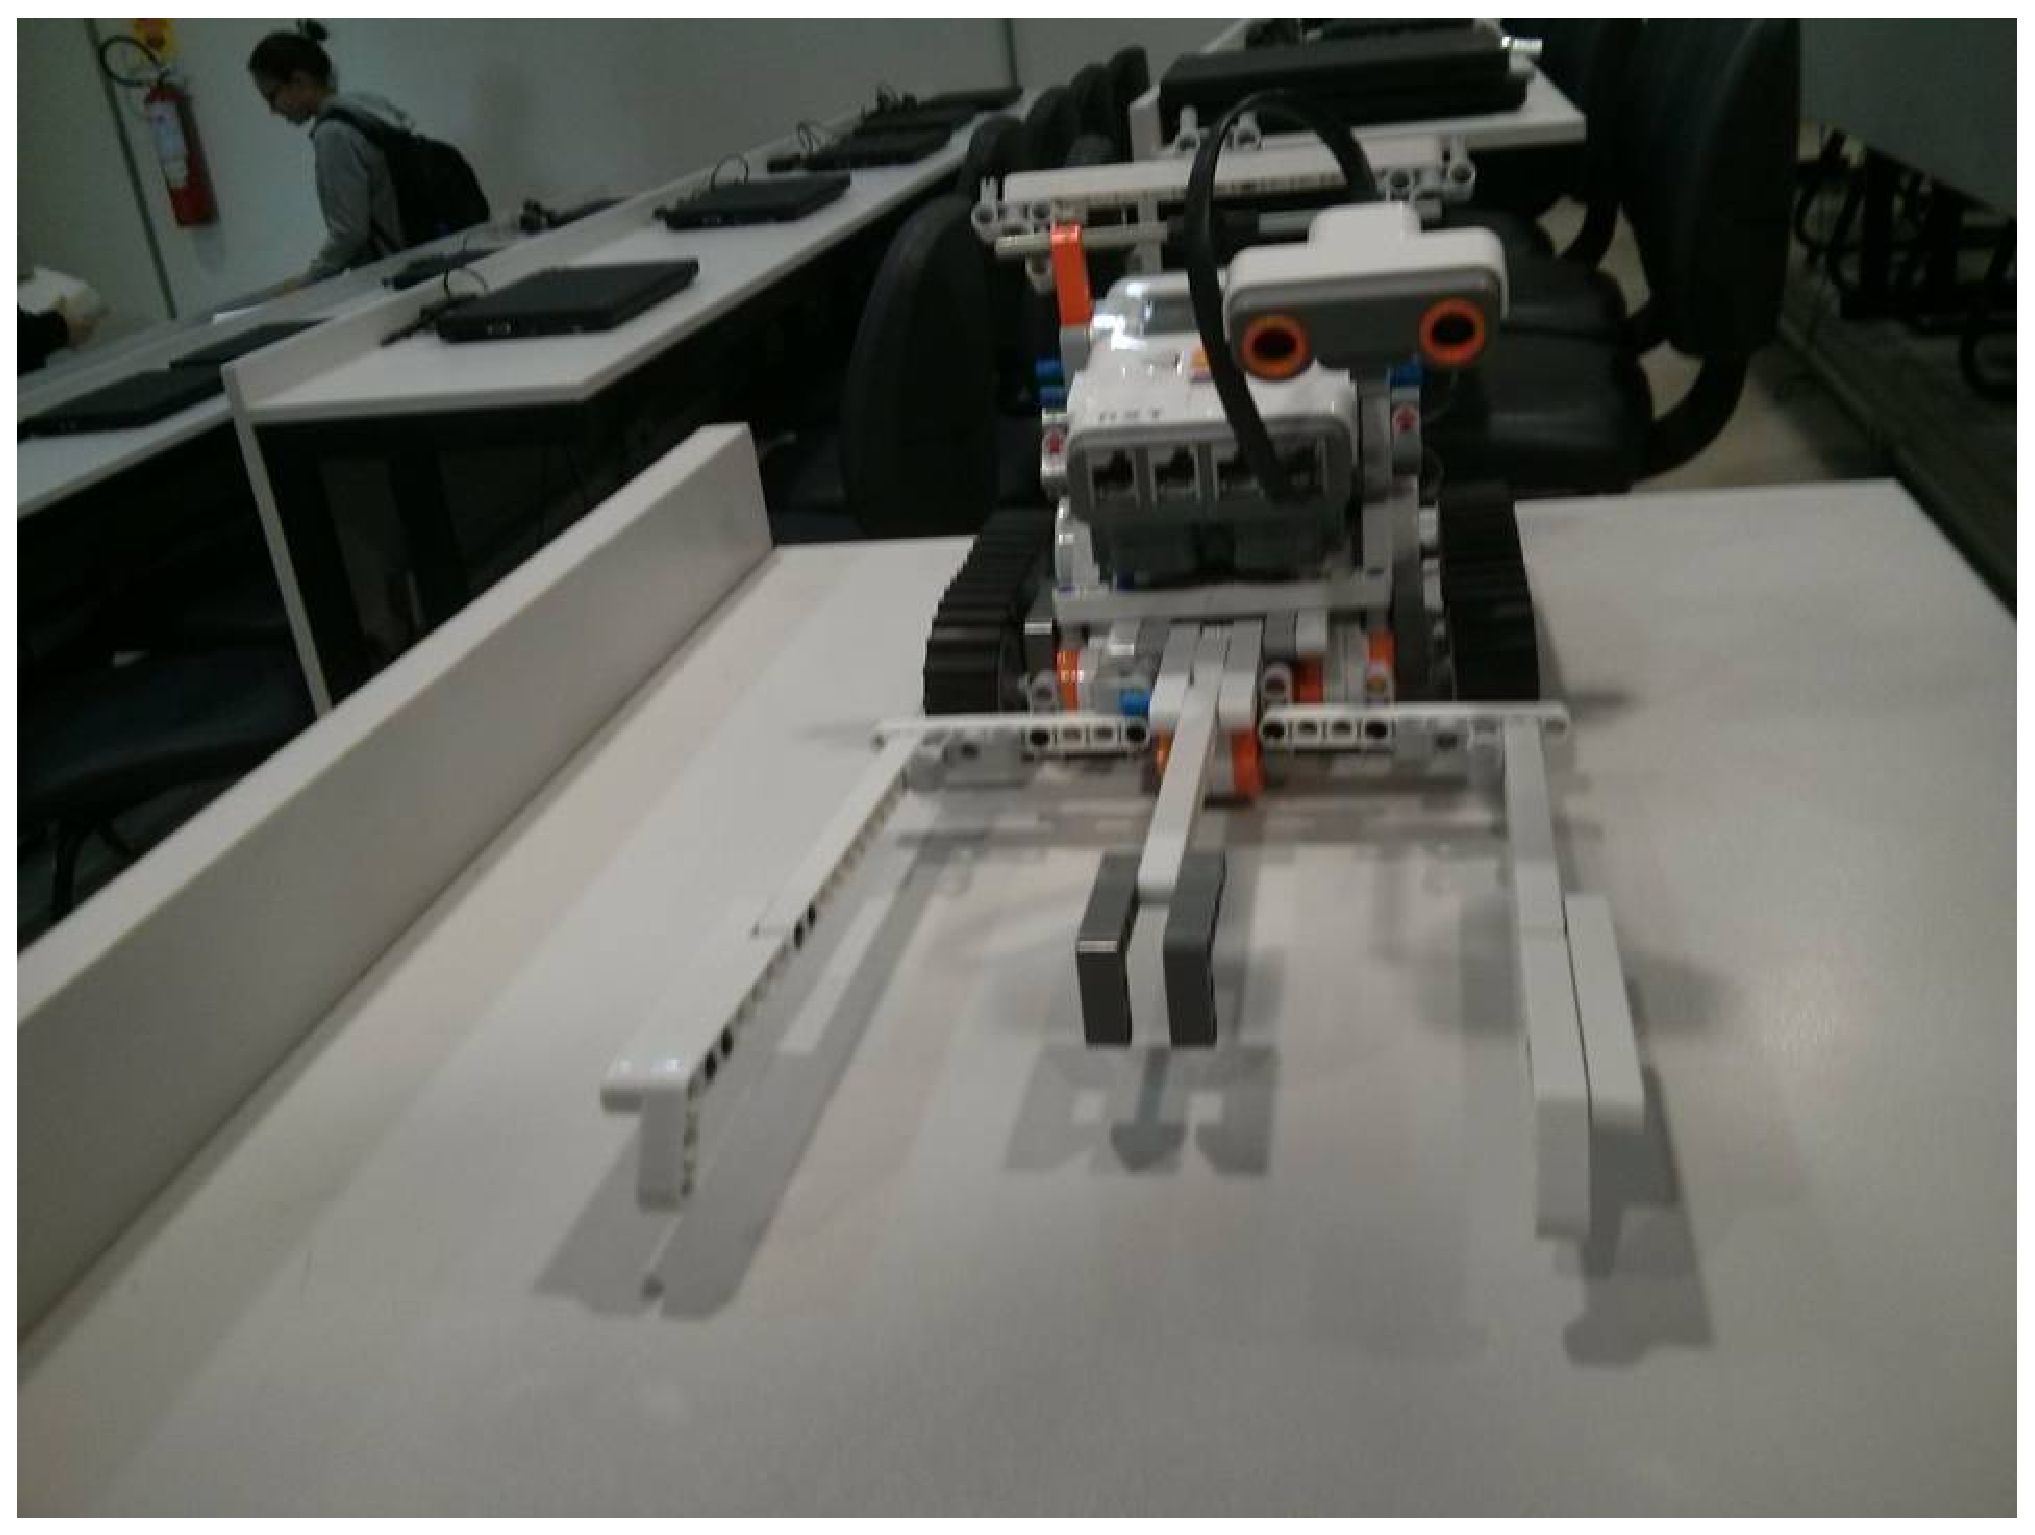
\includegraphics[keepaspectratio=true,scale=0.55]
      {figuras/robo_005.eps}
    \caption{Vista frontal inferior.}
\end{figure}

\begin{figure}[h]
    \centering
    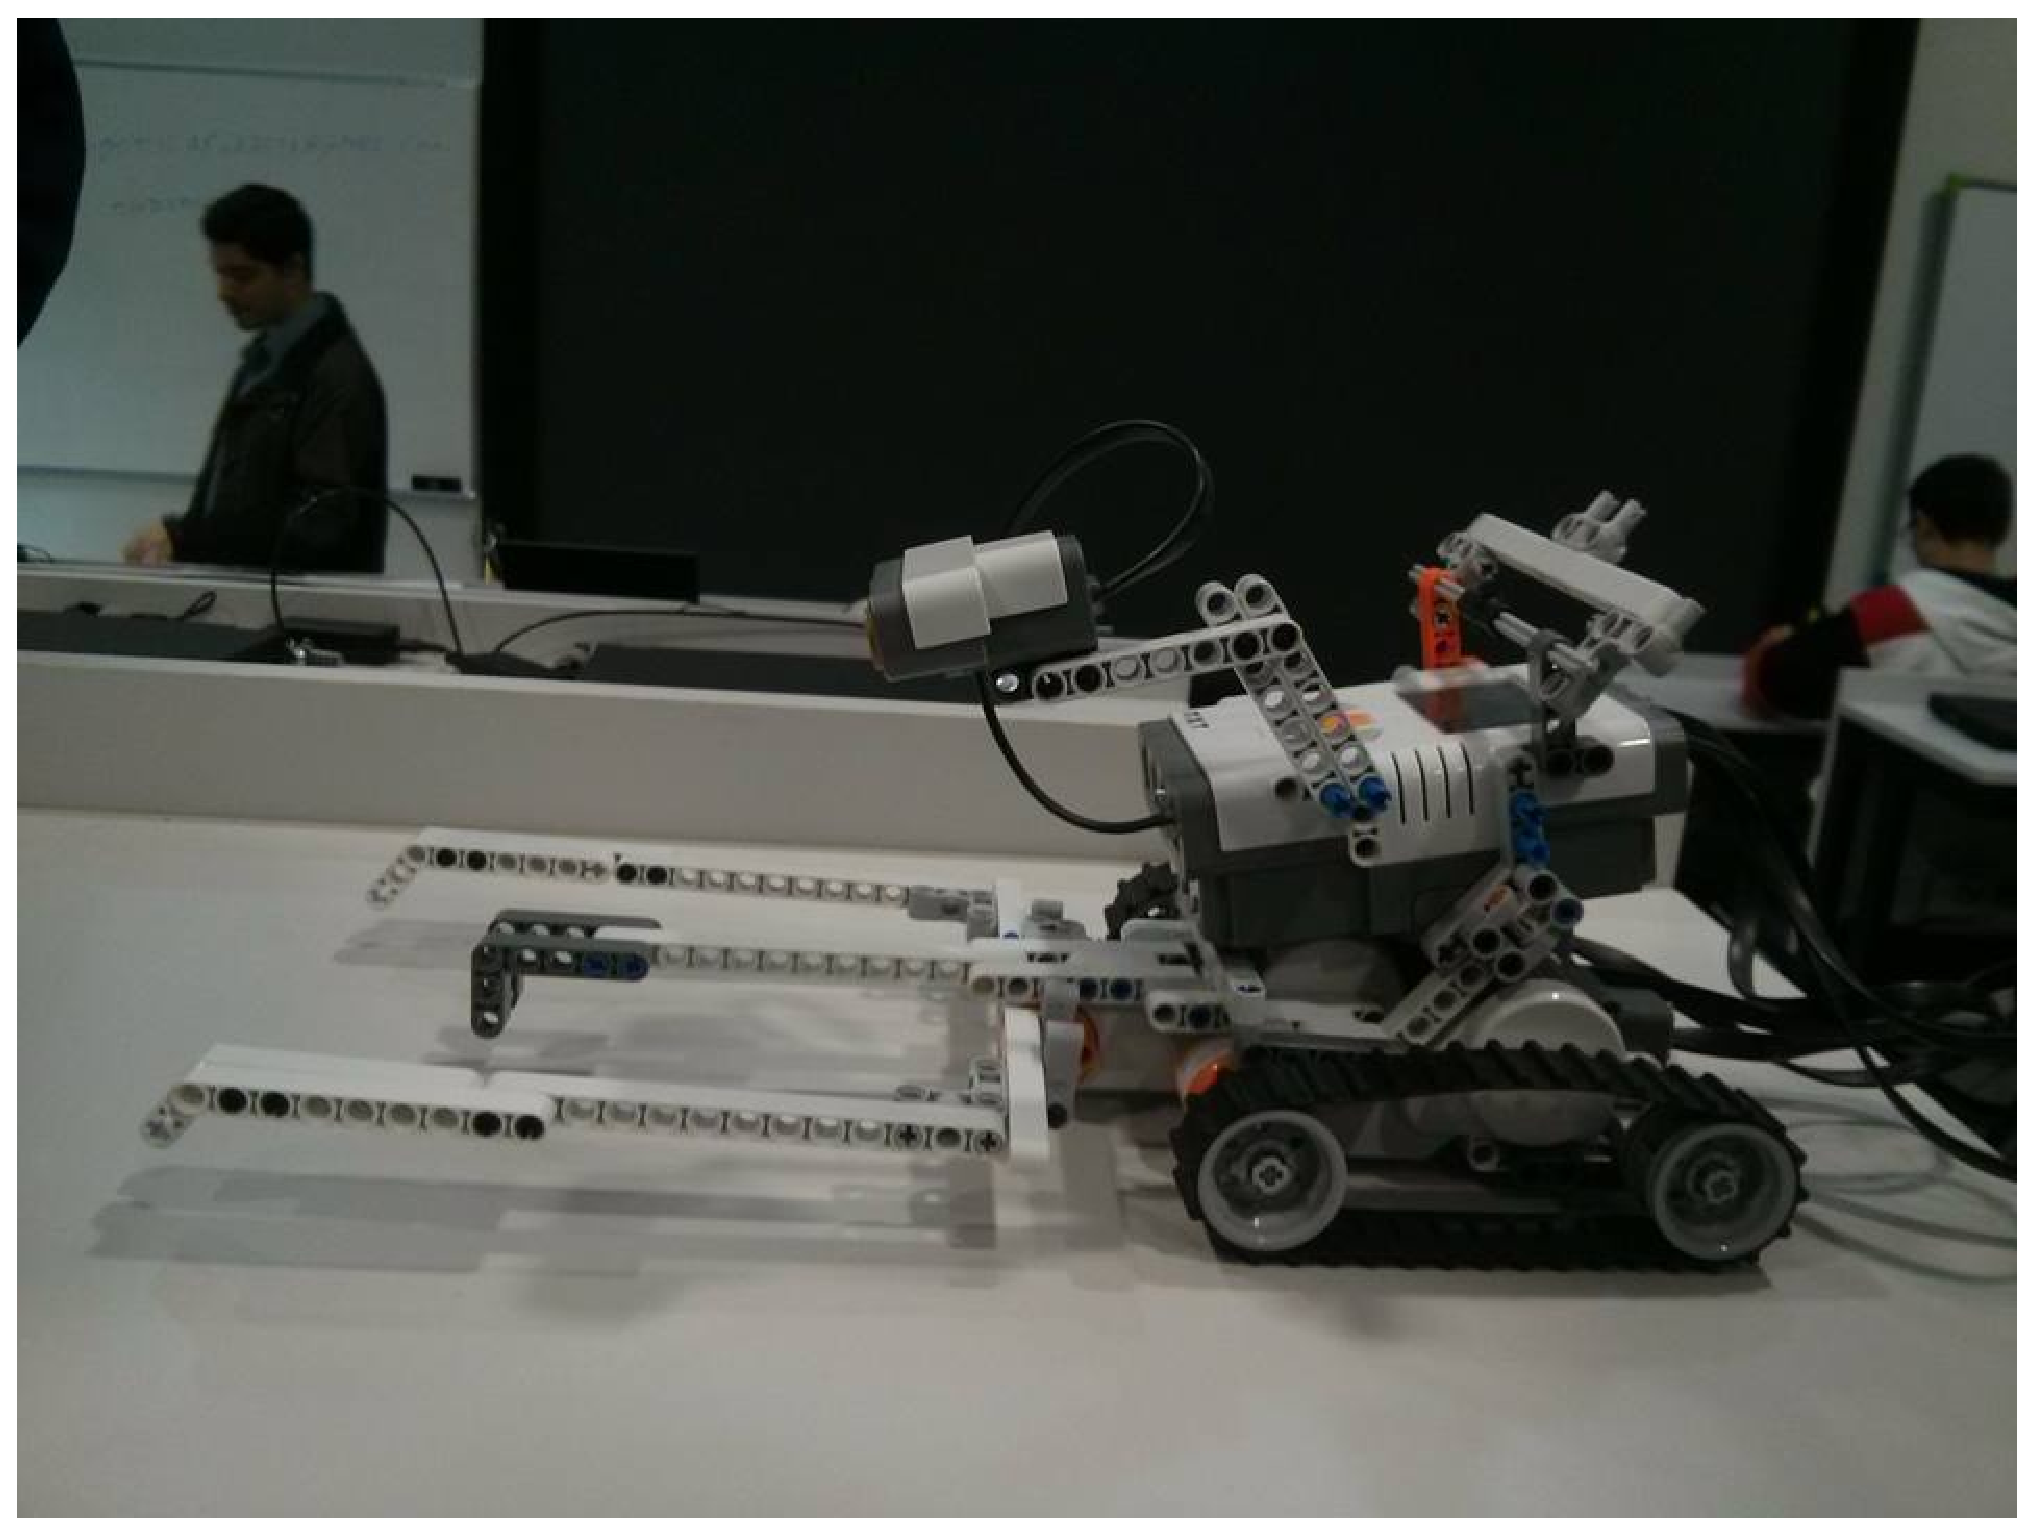
\includegraphics[keepaspectratio=true,scale=0.55]
      {figuras/robo_006.eps}
    \caption{Vista lateral direita.}
\end{figure}

\begin{figure}[h]
    \centering
    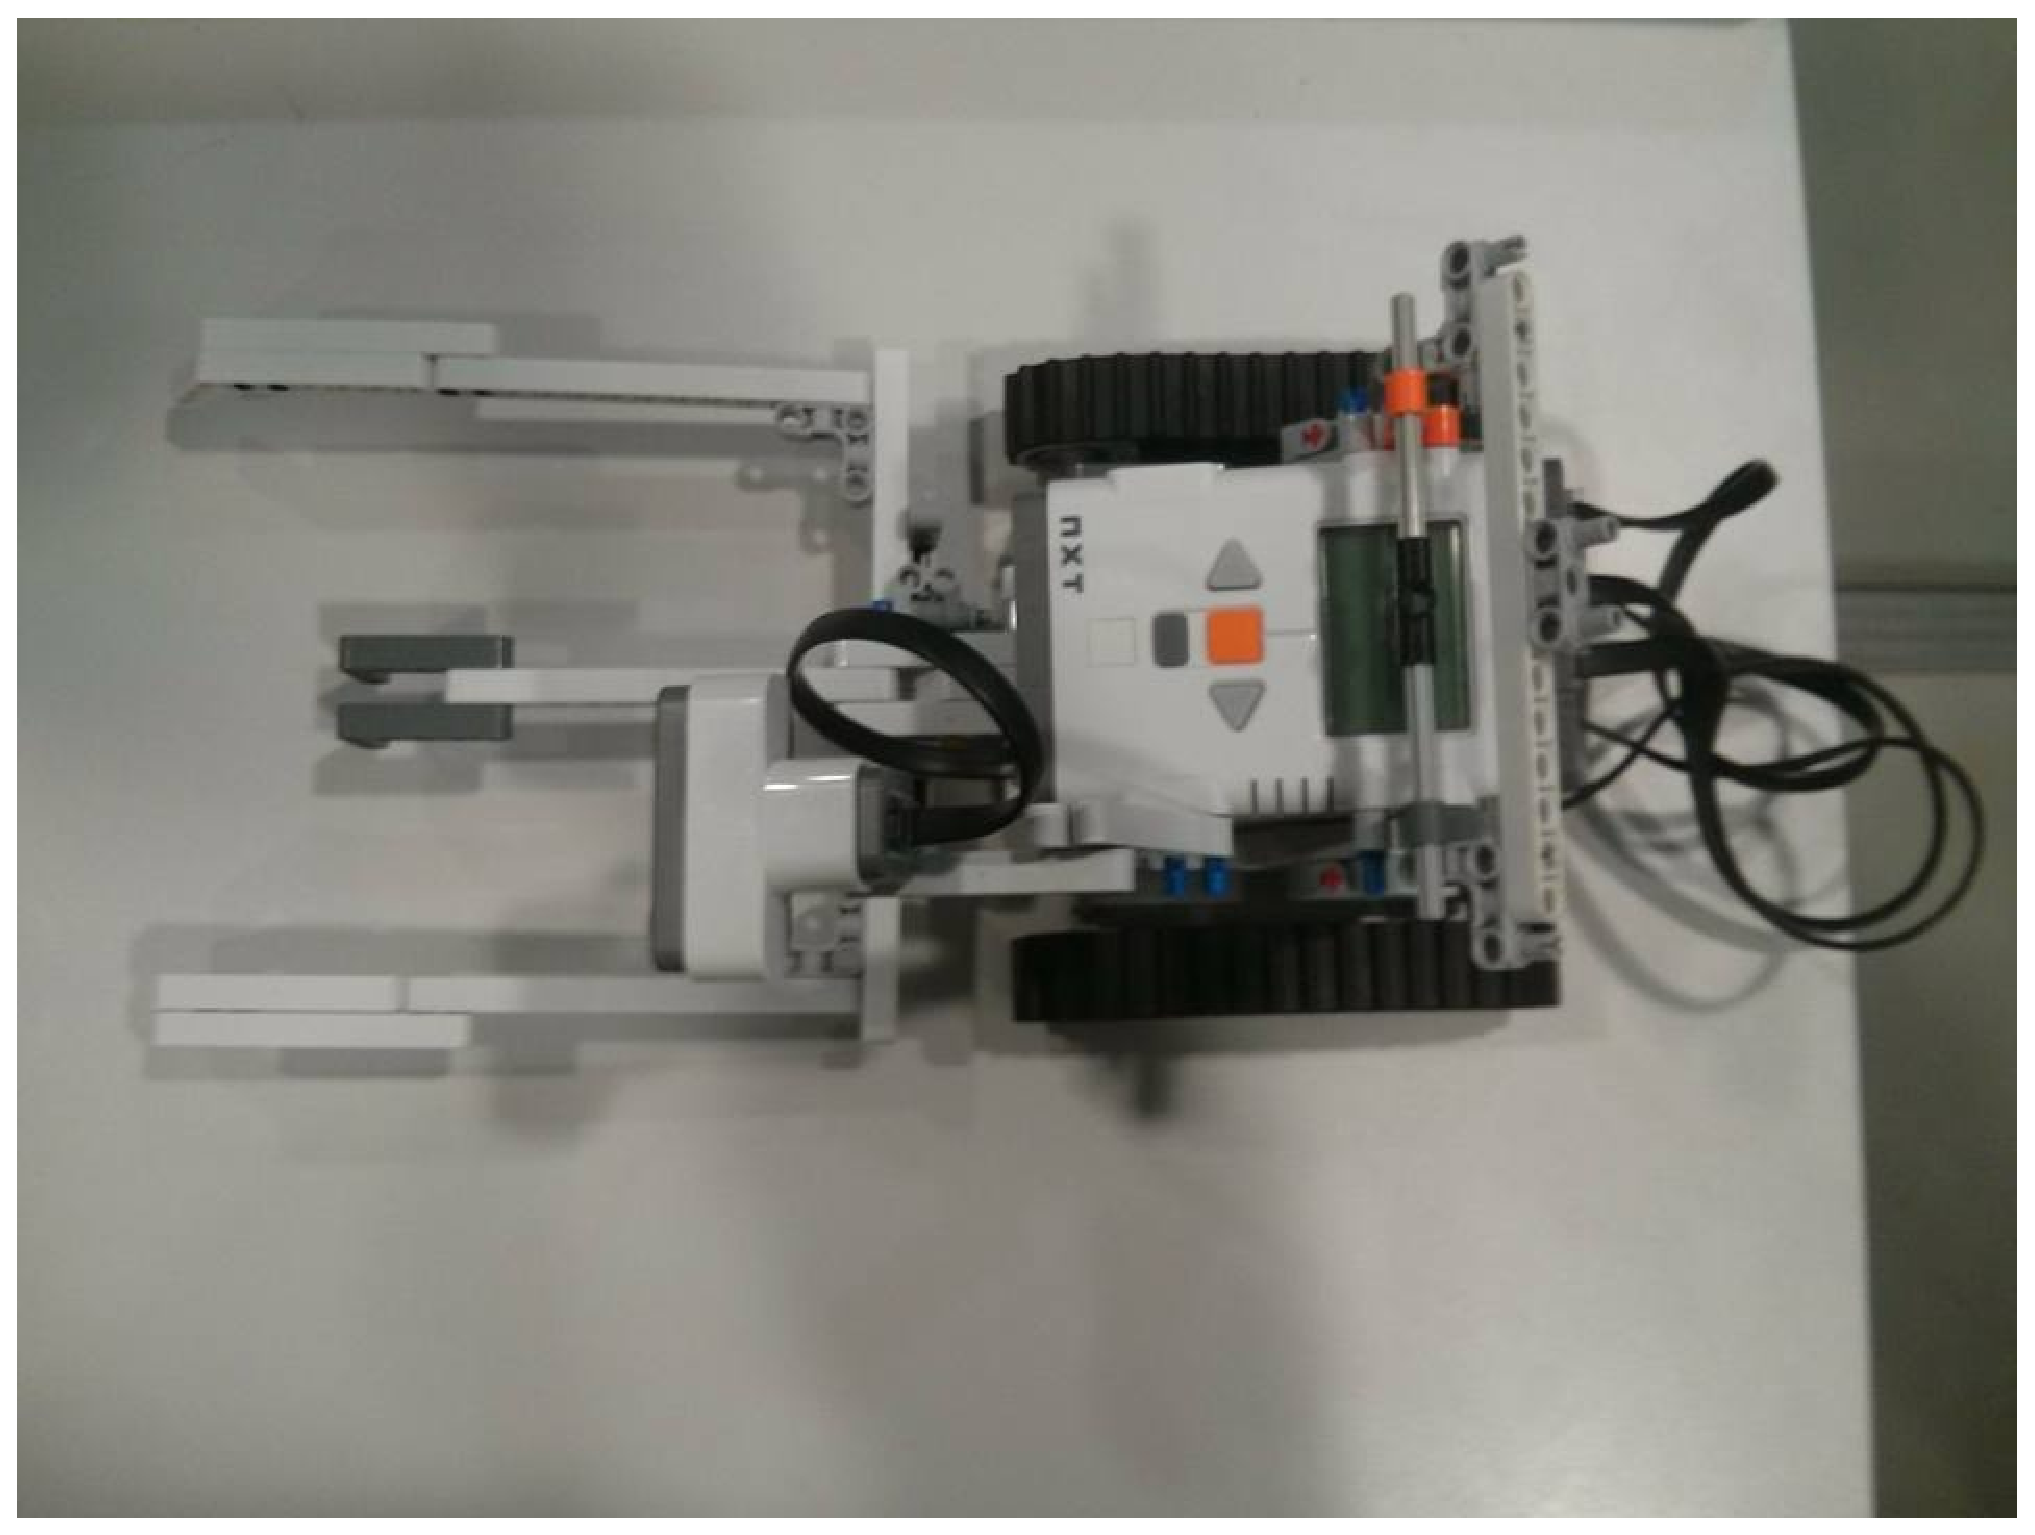
\includegraphics[keepaspectratio=true,scale=0.55]
      {figuras/robo_008.eps}
    \caption{Vista superior.}
\end{figure}

\begin{figure}[h]
    \centering
    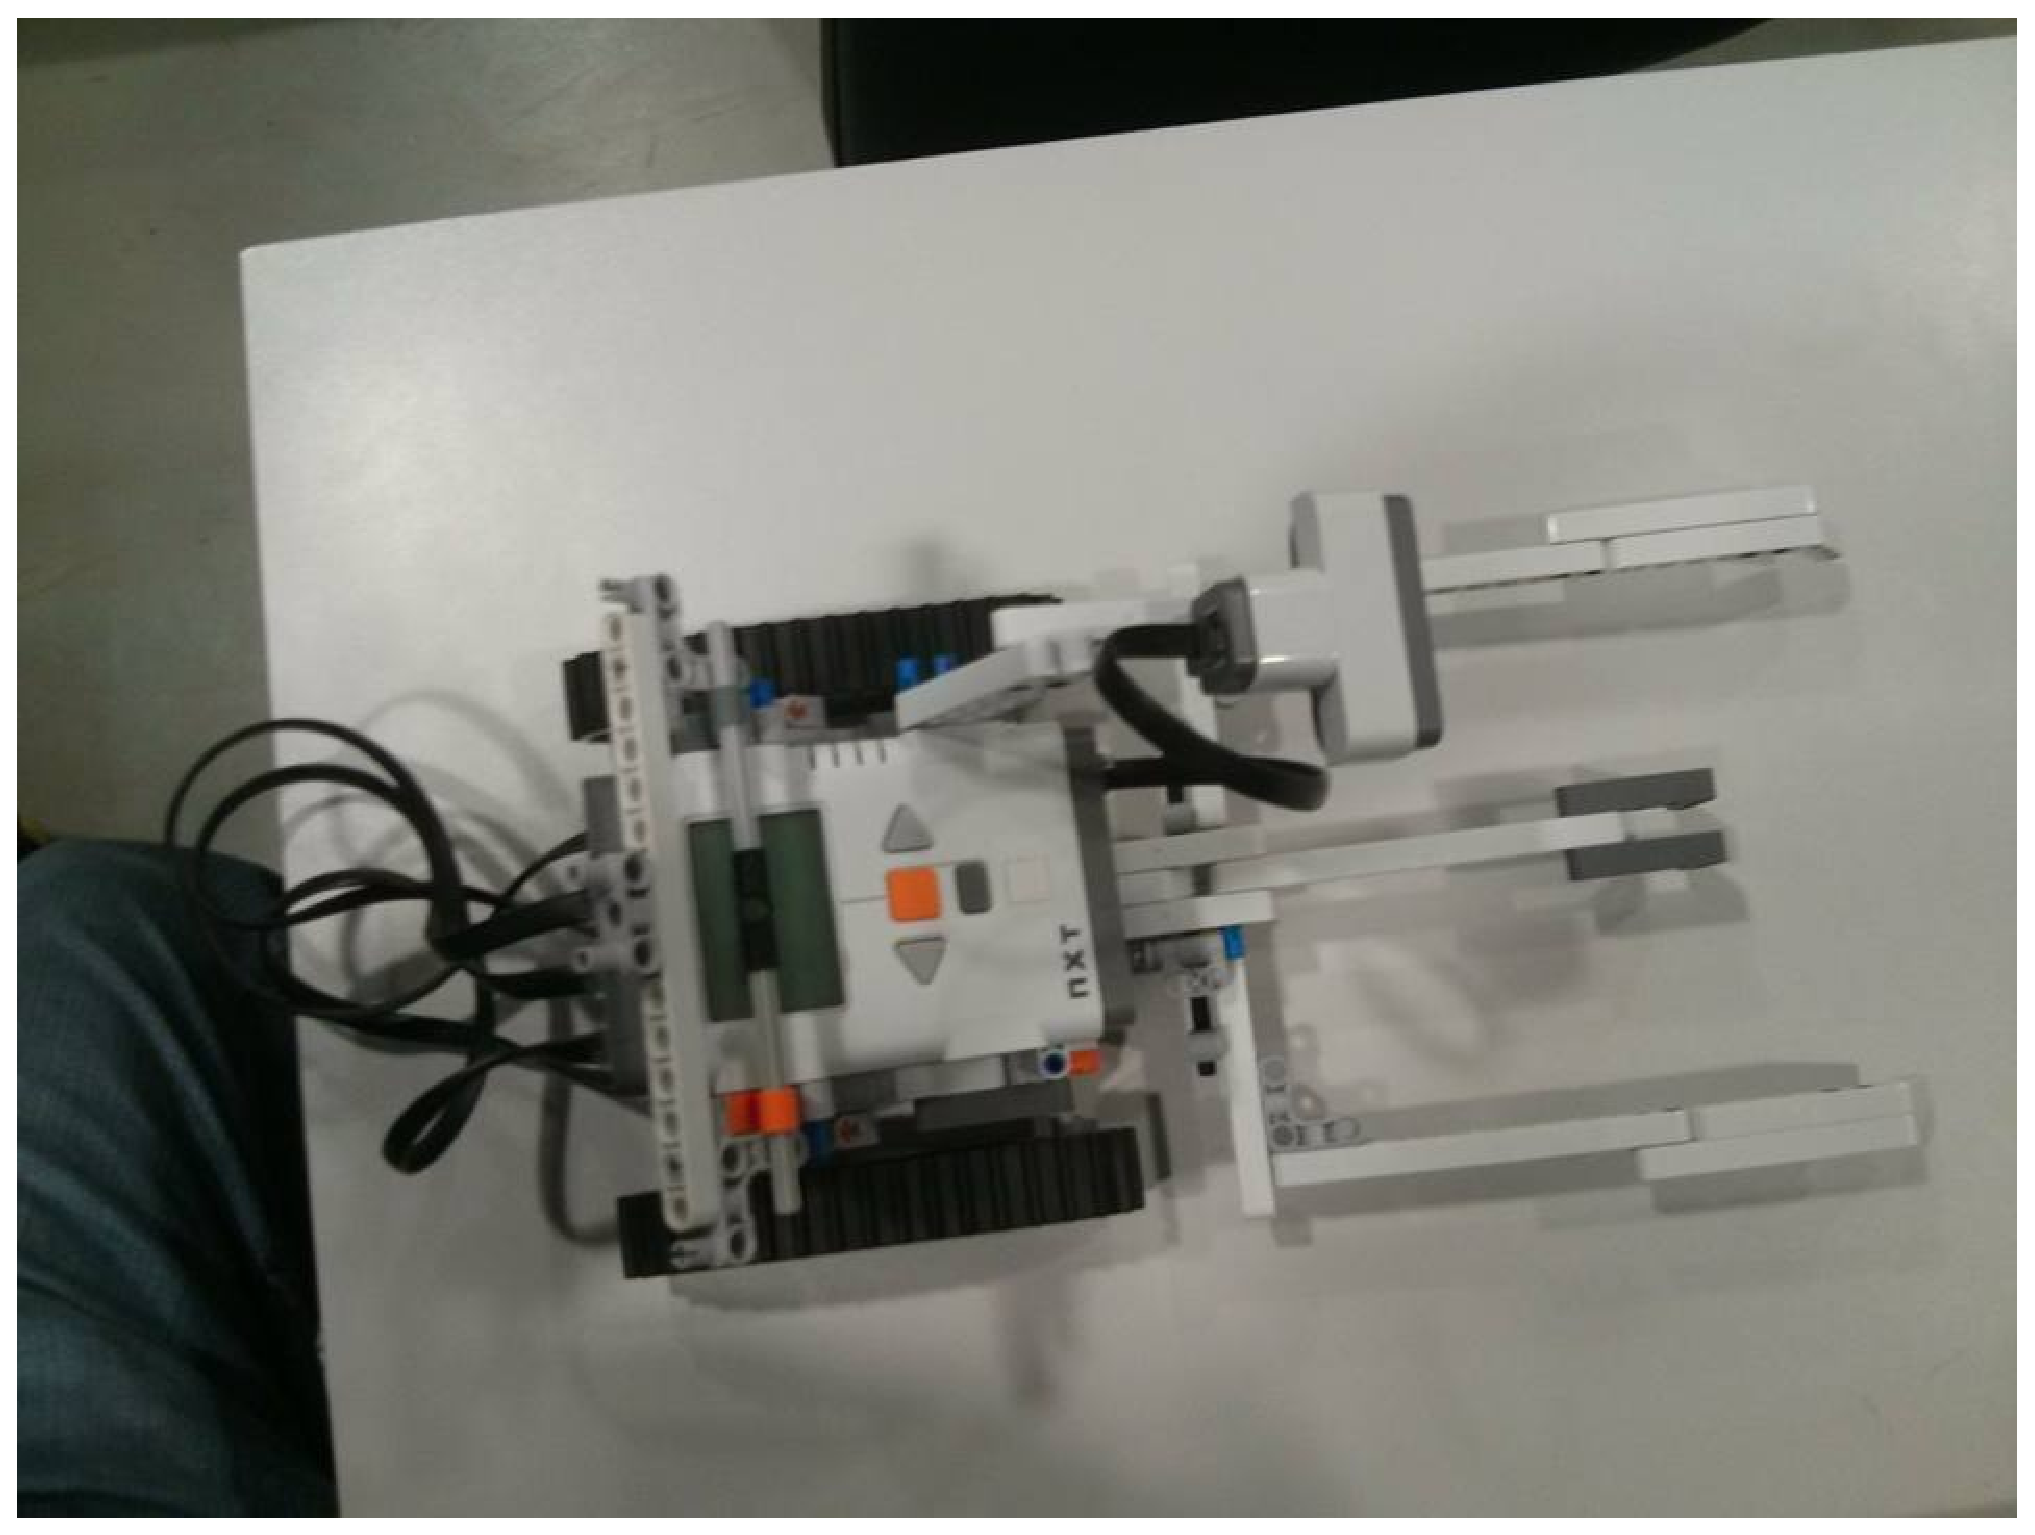
\includegraphics[keepaspectratio=true,scale=0.55]
      {figuras/robo_010.eps}
    \caption{Vista superior com detalhe.}
\end{figure}

\begin{figure}[h]
    \centering
    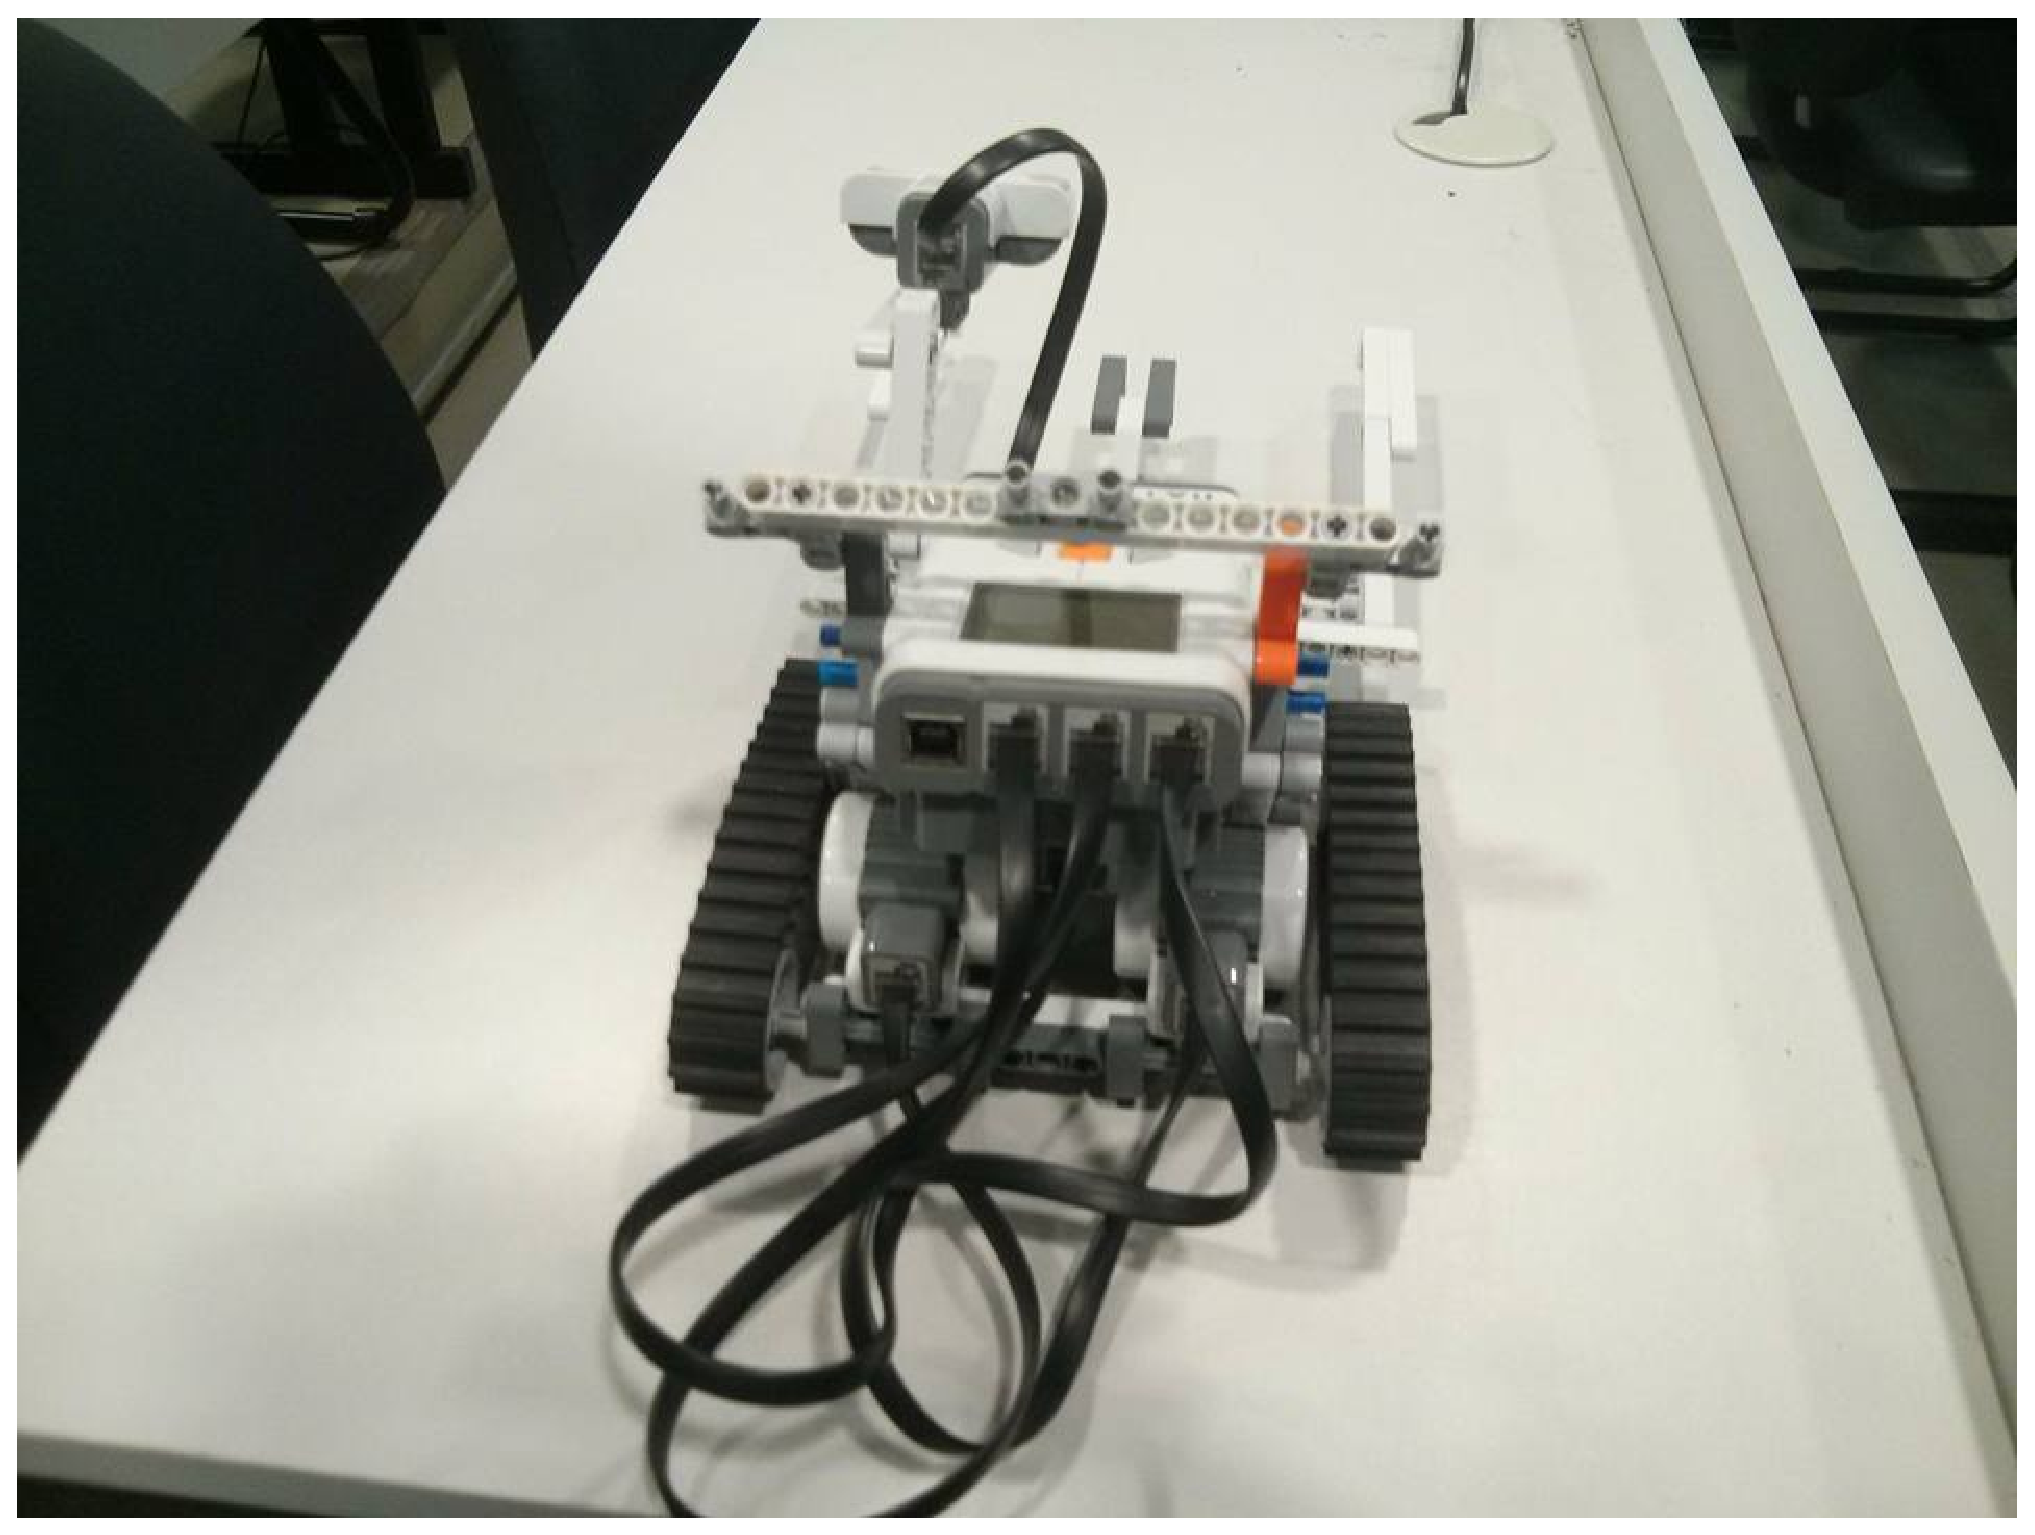
\includegraphics[keepaspectratio=true,scale=0.55]
      {figuras/robo_011.eps}
    \caption{Vista traseira.}
\end{figure}

\end{apendicesenv}
